\begin{frame}[label=Leibniz]
    \frametitle{Leibniz}
    \begin{block}{Nova Methodus}
    Nel 1684 Leibniz diede alle stampe l'opera \textit{Nova Methodus pro maximis e minimis}, 
    la prima pubblicazione sul \alert{calcolo differenziale}  
    inteso nell'accezione moderna: un metodo e un simbolismo generali
    per il calcolo delle tangenti alle curve.
    \end{block}
    \pause
    \begin{block}{Prima esposizione moderna del Calcolo Differenziale}
        Troviamo la notazione $\frac{dy}{dx}$, le regole di differenziazione e il concetto 
        di funzione (anzi la parola stessa). Leibniz introduce la notazione \textit{dx} 
        per denotare un incremento infinitesimo di x (la "d" sta per differenza).
    \end{block}
    \pause
    \begin{exampleblock}{Adesione agli infinitesimi}
        Per esempio se $y = uv$ dove u,v sono funzioni della $x$.
        L'incremento $dy$ diventa:
        \begin{center}
            \scalebox{1.5}{%
            $dy=(u+du)(v+dv)-uv = udv+vdu+ dudv$%
            }
        \end{center}
        e il coefficiente angolare $\frac{dy}{dx}$ della retta che passa 
        per il punto $(x,y)$ e il punto infinitamente vicino $(x+dx,y+dy)$
        si ottiene, a meno di un infinitesimo, semplicemente dividendo per $dx$:
        \begin{center}
            \scalebox{1.5}{%
            $\frac{dy}{dx} =  u\frac{dv}{dx} + v\frac{du}{dx} $%
            }
        \end{center}
    \end{exampleblock}
\end{frame}

\begin{frame}
    \frametitle{L'integrale secondo Leibniz}
    \begin{block}{La definizione}
        Nel 1686 Leibniz da alle stampe la prima pubblicazione 
        sul Calcolo integrale. Introduce la notazione $\int$$ydx$ per indicare
        la funzione $y$ di $x$ , dove $\int$, una S allungata sta per "somma".
        Il termine seguente, $ydx$, indica l'area di un rettangolo infinitesimo 
        di altezza $y$ e base $dx$. 
        Quindi $\int$$ydx$ denota la somma di queste aree infinitesime: 
        l'area sottesa alla curva la cui altezza in $x$ è $y$.  
    \end{block}
    \begin{center}
        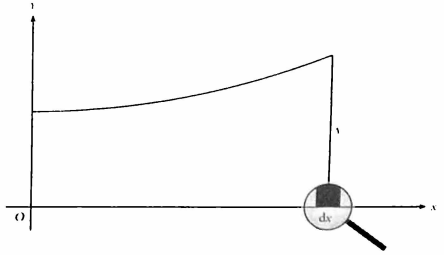
\includegraphics[scale=.6]{Area-somma-rettangoli.png}
    \end{center}
\end{frame}

\begin{frame}
    \frametitle{Il TFC secondo Leibniz}
    \begin{alertblock}{Domanda}
    \begin{center}
        \fontsize{15}{17.2}\selectfont
        Che cosa significa $d$$\int$$ydx$ ?
    \end{center}
    \end{alertblock}
    \begin{block}{Teorema}
        Poiché $d$ significa "\textit{incremento infinitesimo}" e $\int$
        significa "\textit{somma}", allora $d$$\int$$ydx$ significa
        "\textit{incremento Infinitesimo della somma (di infiniti $ydx$} \textit{)}",
        La risposta é sicuramente :
        \begin{center}
        \scalebox{2}{%
                    $d$$\int$$ydx = ydx$%
                    }
        \end{center}
        Quindi
        \begin{center}
            \scalebox{2}{%
            $\frac{d}{dx}$$\int$$ydx = y$%
            }
        \end{center}
        In parole: \textit{Se si integra una funzione $y$ e poi si 
        differenzia il risultato si ottiene di nuovo la funzione $y$
        }
    \end{block}
\end{frame}